%\/\/\/\/\/\/\/\/\/\/\/\/\/\/\/\/\/\/\/\/\/\/\/\/\/\/\/\/\/\/\/\/\/\/\/\/\/\/\/\/\/\/\/\/\/\/\/\/\/\/\/\/\/\/\/\/\/\/\/\/\/\/\/\/\/\/\/\/\/
%				Eliminata
%\/\/\/\/\/\/\/\/\/\/\/\/\/\/\/\/\/\/\/\/\/\/\/\/\/\/\/\/\/\/\/\/\/\/\/\/\/\/\/\/\/\/\/\/\/\/\/\/\/\/\/\/\/\/\/\/\/\/\/\/\/\/\/\/\/\/\/\/\/		


		\begin{frame}{Meccanica Geometrica}
  			\begin{columns}[T]
    			\begin{column}{.5\textwidth}		
					\begin{itemize}
						\item \textbf{L'Idea:} Fare uso della geometria per codificare tutte le proprietà meccaniche di un sistema indipendentemente dalle coordinate di configurazione.(Lessig)
						\item \textbf{La scommessa:} Saper ricostruire da questi oggetti matematici astratti tutte le osservabili di interesse fisico.
						\item \textbf{Il vantaggio:} Base formale su cui definire la Quantizzazione.
					\end{itemize}
    			\end{column}
    		   	\begin{column}{.5\textwidth}
							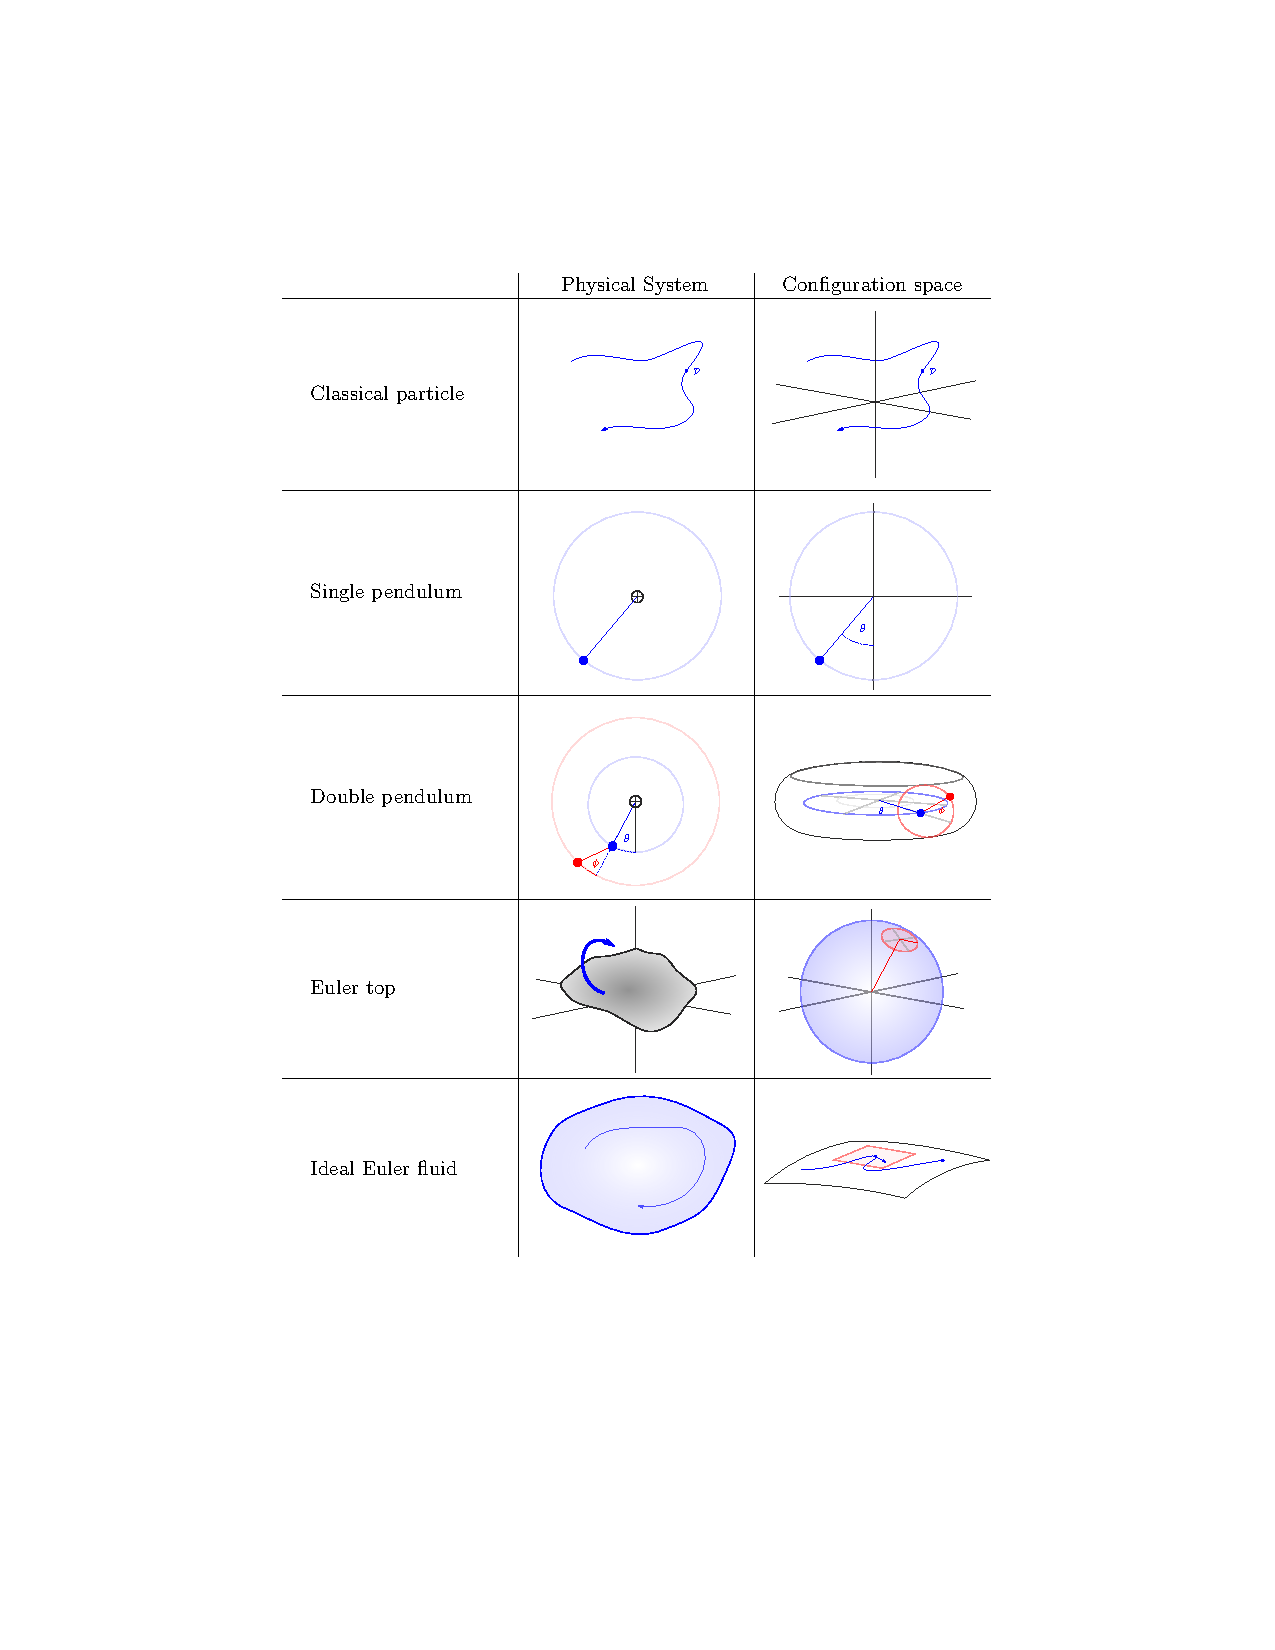
\includegraphics[width=\textwidth]{Presentazione/GeoMec_Crop} 				
    			\end{column}
  			\end{columns}	
	\end{frame}

		\begin{frame}	
			\frametitle{Formalismo Canonico Covariante}
  			\begin{columns}[T]
    			\begin{column}{.5\textwidth}
    				\comment{ Facciamo un Cambio di prospettiva: non più conformazioni "statiche" ma considero tutti i moti possibili}
					\begin{itemize}
						\item Spazio delle configurazioni cinematiche $\Conf$ \comment{è l'insieme di tutte i moti compatibili con la cinematica}
						\item Dinamica codificata dall'azione $S:\Conf \rightarrow \Real$ \comment{l'azione la rivediamo come una mappa definita sui moti}
						\item Equazioni differenziali del moto $ P$ \comment{ dal principio di minima azione discende un'equazione differenziale su $\Conf$}
						\item Spazio delle configurazioni dinamiche $\Sol$ \comment{Insieme delle equazioni del moto}		
					\end{itemize}
					\vspace{5mm}
					\onslide<6>{Perchè non cambiare \emph{Pittura?} 
						\comment{\\accenno: quello che si sta facendo ricorda in un certo senso il passaggio dalla pittura di schrodinger a quella di heisnberg}
						\comment{\\difficoltà: queste varietà sono infinito dimensionali}					
					}

    			\end{column}

    		   	\begin{column}{.5\textwidth}
					\parbox[c][.7\textheight][c]{\columnwidth}{%
						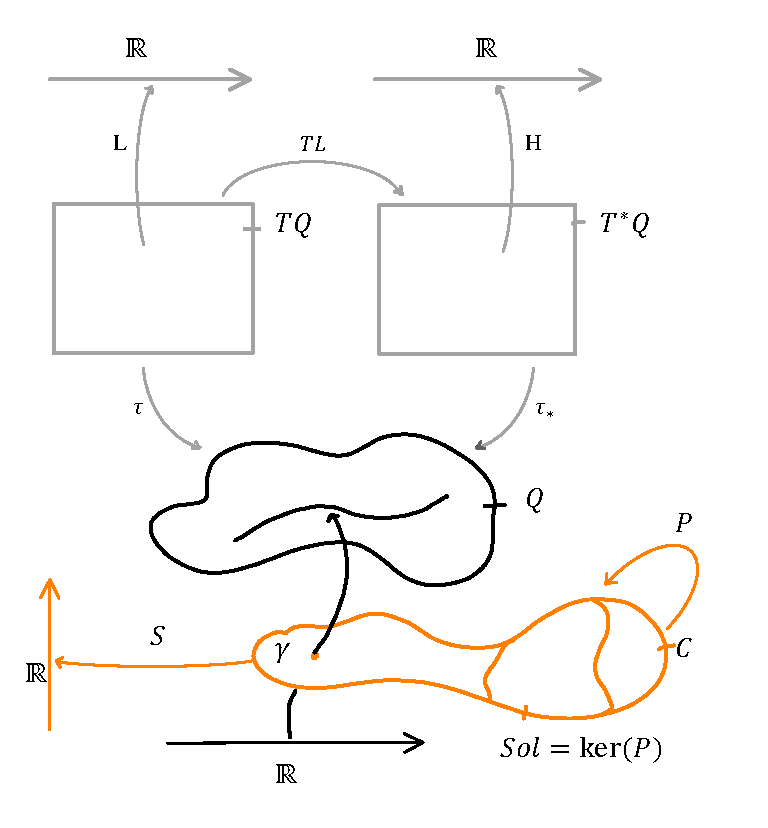
\includegraphics [width=\textwidth]{Presentazione/GeoMecFrameB} 
					}
    			\end{column}
  			\end{columns}		
		\end{frame}


		\begin{frame} 	% \danger : manca overlay: popup graduale degli elementi
			\frametitle{Recuperare il formalismo canonico non covariante \comment{(Eliminare?)\bomb}}		
  			\begin{columns}[T]
    			\begin{column}{.5\textwidth}
					Osservazione chiave: lo spazio delle fasi ordinario è uno spazio di \emph{Dati iniziali}
					\begin{itemize}
						\item<1-> Definiamo $\Data$ = spazio dei dati iniziali \comment{nota tecnica, perchè si possa fare il base space $M$ deve ammettere delle superfici di cauchy: Servono spazitempi globally hyperbolic}
						\item<2-> Definiamo $\SolMap$ che associa ad ogni dato l'unica soluzione
					\end{itemize}
    			\end{column}
    		   	\begin{column}{.5\textwidth}
					\comment{Wip: un immagine indicativa potrebbe essere quella del campo di calore ad esempio sulla superficie terreste. Noto il profilo di calore sulla superficie si può calcolare la soluzione}
						%\includegraphics<1> [width=\textwidth]{Pictures/FieMecFrame}
    			\end{column}
  			\end{columns}		

		\end{frame}

		\begin{frame}	% \danger : manca overlay: popup graduale degli elementi
			\frametitle{Formalismo Covariante esteso ai Campi}
  			\begin{columns}[T]
    			\begin{column}{.5\textwidth}
    				\comment{Il formalismo covariante intrinseco si estende facilmente a sistemi più generali!\\}
    				L'idea
    					\begin{itemize}
    						\item fondamento della cinematica non $Q$ ma $\Real \times Q$ (fibrato di configurazione) 	\comment{triviale nel caso dei sistemi ordinari}
    						\item Le configurazioni cinematiche 
    							\begin{displaymath}
    								\underset{(\textrm{curve})}{\gamma: \Real \rightarrow Q} \quad \mapsto \quad 
    								\underset{(\textrm{sezioni})}{\gamma: \Real \rightarrow Q\times \Real}
    							\end{displaymath}
    					\end{itemize}	

    				\begin{block}<2->{Per  i campi}
 						\begin{itemize}
							\item Fibrato di configurazione \comment{Ingloba la struttura Cinematica}
								\begin{itemize}
									\item[$\cdot$]  Sezioni = Spazio delle configurazioni cinematiche 
								\end{itemize}
							\item Densità Lagrangiana \comment{ingloba la struttura dinamica}
								\begin{itemize}
									\item[$\cdot$] Equazioni di Eulero-Lagrange determinano operatore del moto $P$
									\item[$\cdot$] Soluzioni di P = Spazio delle configurazioni dinamiche
								\end{itemize}
						\end{itemize}   				
    				\end{block}
    			\end{column}
    		 
    		   	\begin{column}{.5\textwidth}
					\comment{Evidenziare uno alla volta gli oggetti che introduco}
						\includegraphics<1> [width=\textwidth]{Pictures/FieMecFrame} 
						\includegraphics<2-> [width=\textwidth]{Presentazione/AbstractFieldTheory(pezzotta)} 
    			\end{column}
  			\end{columns}		
		\end{frame}


		\begin{frame}
			\frametitle{A che punto siamo?  \comment{(Eliminare?)\bomb}}	
			\begin{itemize}
				\item Abbiamo identificato due spazi candidati a rappresentare \emph{lo spazio delle fasi di una teoria di campo classica}
					\begin{itemize}
						\item $\Data$: insieme dei possibili dati iniziali 
						\item $\Sol$: insieme delle soluzioni delle equazioni del moto
					\end{itemize}
					 	\comment{notare che $\Data$ si identifica con lo spazio delle fasi ordinario $T^*Q$ per via del suo rapporto biunvoco con lo spazio delle soluzioni.}
				\item Manca la dotazione di una forma simplettica \comment{notare che per il caso c'era una scelta naturale: teorema di darboux o dal punto di vista intrinseco: tautological 1-form}
				\item Manca l'identificazione di un'algebra di Poisson di \emph{osservabili classici}
			\end{itemize}
			
			\begin{block}{Soluzioni}
				I metodi per equipaggiare una teoria di campo  di una struttura simplettica  sono molteplici:
				\begin{itemize}
					\item via lo spazio dei Dati (Wald)
					\item via lo spazio delle Soluzioni (Crnkovic, Witten , ...)
					\item il metodo di Peierls
					\item \comment{altri ?}			
				\end{itemize}
			\end{block}
		\end{frame}

	\begin{frame}
		\frametitle{I passi del metodo di Peierls (1) \comment{(Eliminare? -> solo voce?)\bomb}}	
			La procedura può essere riassunta in pochi passi:
		\begin{enumerate}
			\item Si considera un disturbo Lagrangiano$\chi$. \comment{that is a time-compact Lagrangian density}
				\begin{displaymath}
					\chi in
				\end{displaymath}
			\item Si costruiscono le soluzioni perturbate dall'azione di $\chi$.
			\item Si calcolo l'effetto del disturbo $\chi$ sul funzionale Lagrangiano relativo ad un secondo disurbo $\omega$.
			\item Si assembla l'effetto reciproco dei due disturbi a costruire una funzione binaria.
		\end{enumerate}	
	\end{frame}

	\begin{frame}
		\frametitle{I passi del metodo di Peierls}
			Per semplicità rappresentiamo lo spazio infinito dimensionale $\Conf$ come un piano.
		  	\begin{columns}[T]
    			\begin{column}{.5\textwidth}
						\begin{enumerate}
							\item<2->  Alla  Lagrangiana disturbata corrisponde un proprio spazio di soluzioni.
							\item<3-> Si determinano tra tutte le possibili variazioni $\phi_\epsilon$ di $\phi_0$ quelle che ricadono in $\Sol_\epsilon$ al primo ordine in $\epsilon$
							\item<4-> L'effetto è la derivata del valore di un funzionale $B$ lungo le variazioni appena trovate.
							\item<5-> La parentesi di Peierls si ottiene per confronto dei due effetti anticipato e ritardato:
								\begin{displaymath}
									\{\chi, \omega \}(\phi_0) =
									 \EffectOp_\chi^- \mathcal{O}_\omega (\phi_0) - \EffectOp_\chi^+ \mathcal{O}_\omega(\phi_0)
								\end{displaymath}

							\item<6-> Nel caso di funzionali Lineari l'espressione si semplifica
								\begin{displaymath}
									\{\chi, \omega \}(\phi_0) =
									 \mathcal{O}_\omega (\eta_{-} - \eta_{+})
								\end{displaymath}
						\end{enumerate}
    			\end{column}
    		   	\begin{column}{.5\textwidth}
								\includegraphics<1>[width=\textwidth]{Pictures/GeometricPicture0}
								\includegraphics<2>[width=\textwidth]{Pictures/GeometricPicture1}
								\includegraphics<3>[width=\textwidth]{Pictures/GeometricPicture2}								
								\includegraphics<4-5>[width=\textwidth]{Pictures/GeometricPicture3}
								\includegraphics<6>[width=\textwidth]{Pictures/GeometricPictureLinear1}
								
    			\end{column}
    		\end{columns}
	\end{frame}

	\begin{frame}{L'Algebra di Poison realizzata tramite il metodo di Peierls}
		Risultato:\\
		Alla generica teoria lagrangiana di campo $(E, \Lagrangian)$\\
		Viene associato lo spazio simplettico  $(\Obs, \tau)$ 
		\begin{itemize}
			\item $\Obs \simeq \frac{\Gamma_0}{P \Gamma_0} $
			\item $\tau( [\chi], [\omega]) = \{\chi , \omega \} =\int_M \left\langle\chi, \left(\GreenAdv - \GreenRet \right)\omega \right\rangle 
			d\mu(x) = ( \chi, E \omega) \qquad \forall \chi,\omega \in \Gamma_0(E)$
		\end{itemize}
		\comment{SI prende il quoziente per garantire che la forma sia non degenere\\} 		

		\vfill

		Gli elementi di $\Obs$ agiscono come osservabili:
				\begin{displaymath}
				 F_{[f]}(X) = F_f (X)= \int_M <X, f>_x d\mu(x) \qquad \forall X \in \Sol
				\end{displaymath}
		La forma $\tau$ può essere rivista come una parentesi di Poisson
				\begin{displaymath}
				 \left\{ F_{[f]},  F_{[g]} \right\} (X) = F_{[???]}(X)
				\end{displaymath}
				\comment{adesso mi sfugge}
			
	\end{frame}

	\begin{frame}
		\frametitle{Un esempio: I Campi di Jacobi su flat FRW}
		  	\begin{columns}[T]
    			\begin{column}{.5\textwidth}
					bu
    			\end{column}
    		   	\begin{column}{.5\textwidth}
					bu
    			\end{column}
    		\end{columns}
	\end{frame}	
	
	\begin{frame}
		\frametitle{Un altro esempio: Il campo di Jacobi 1D}
		  	\begin{columns}[T]
    			\begin{column}{.5\textwidth}
					bu
    			\end{column}
    		   	\begin{column}{.5\textwidth}
					\includegraphics<1>[width=\textwidth]{Pictures/Jacobi1D_GeometricPicture0}
					\includegraphics<2>[width=\textwidth]{Pictures/Jacobi1D_GeometricPicturePanoramica}	
    			\end{column}
    		\end{columns}
	\end{frame}	


	\begin{frame}{Conclusioni}
			\begin{itemize}
				\item visto due costruzioni differenti \comment{(Peierls, Dati Iniziali)} per lo spazio simplettico delle teorie di campo classico.
				\item Le due costruzioni sono equivalenti \comment{simplettomorfe} solo in casi particolari.
				\item Entrambe le costruzioni sono esoteriche e calate dall'alto. 
					\comment{ Usate puramente come "black box" per ottenere una forma simplettica utile}:
						\begin{itemize}
							\item a priori non c'è nessun motivo per cui le forme simplettiche che forniscono siano quelle "giuste".
							\item I singoli passaggi della costruzione non hanno giustificazione fisica.
						\end{itemize}
					\comment{ sappiamo il come, sappiamo che funziona ma non sappiamo "perchè"}
			\end{itemize}
			
		\begin{block}{Perchè focalizzarsi sul campo di Jacobi?}
			\begin{itemize}
				\item
					In questo caso la costruzione di Wald non è ambigua. \\
					 Data è isomorfo a $\Real^{2N}$ e la forma $\Sigma$ che viene imposta dalla procedura di Wald corrisponde all'unica scelta possibile prevista dal teorema di Darboux
					 \comment{\\ (notare che anche per il semplice campo scalare lo spazio data è costituto da coppie di funzioni $C_0$ tutt'altro che finito dimensionale.)}
				\item Ci si può porre il problema di trovare un interpretazione geometrica.\\
				 Perchè la costruzione di Peierls fornisce proprio la giusta usuale forma simplettica (parentesi $\Omega$) sullo spazio delle fasi classico?
				
			\end{itemize}		
		\end{block}
	\end{frame}